\section{Theorie}
\label{sec:Theorie}

Fast alle räumlich und zeitlich periodischen Vorgänge können durch die Sinusfunktion
und die Cosinusfunktion dargestellt werden.
\begin{align}
  f_s(t) &= a \cdot \symup{sin}\left(\frac{2\pi}{T}t\right) \\
  f_c(t) &= b \cdot \symup{cos}\left(\frac{2\pi}{T}t\right).
\end{align}
a und b sind die Amplituden der Wellen und T die Periodendauer.

Diese Aussage folgt aus dem Fourierschen Theorem. Dieses besagt: Konvergiert die Reihe
\begin{equation}
  \frac{a_0}{2} + \sum_{n=1}^\infty \left(a_n \cdot \symup{cos}\left(\frac{2\pi}{T}t\right) + b_n \cdot \symup{sin}\left(\frac{2\pi}{T}t\right) \right)
\end{equation}

gleichmäßig, so stellt sie eine periodische Funktion $f(t)$ dar. Für die Koeffizienten $a_n$ und $b_n$ gilt:

\begin{align}
  a_n &= \frac{2}{T} \int_{0}^{T} f(t) \cdot \symup{cos}\left(\frac{2\pi n}{T}t\right) \, \symup{d}t \\
  b_n &= \frac{2}{T} \int_{0}^{T} f(t) \cdot \symup{sin}\left(\frac{2\pi n}{T}t\right) \, \symup{d}t
\end{align}

Für eine Grundfrequenz $\nu_1 = \frac{2\pi}{T}$ treten in der Fourierreihe nur ganzzahlige vielfache dieser
Frequenz auf. Diese werden als Oberschwingungen bezeichnet

Wird die Amplitude der Schwingungen gegen ihre Frequenz aufgetragen, ergibt sich ein
Linienspektrum wie in Abbildung 1.

\begin{figure}[H]
  \centering
  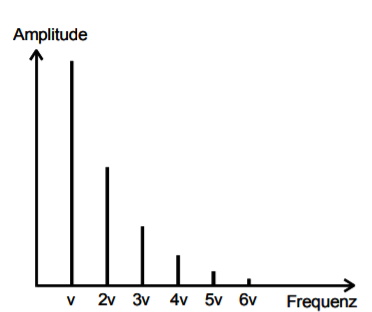
\includegraphics[height=5cm]{Linienspektrum.PNG}
  \caption{Linienspektrum einer periodischen Funktion. \cite{sample}}
  \label{fig:Linienspektrum}
\end{figure}

$n$ geht für $\nu \to \infty$ gegen Null.
Hat die Funktion $f(t)$ Sprungstellen $t_0$ kann die Fourierreihe $f$ dort nicht approximieren. Es kommt zu einer
Abweichung, welche auch für größere $n$ nicht kleiner wird. Dies ist das Gibbs'sche Phänomen.

\subsection{Fourier-Transformation}
Die Fourier-Transformation transformiert eine zeitabhängige Funktion $f(t)$ in dessen Frequenzspektrum $g(\nu)$. Es gilt:
\begin{equation}
  g(\nu) = \int_{-\infty}^{\infty} f(t) e^{i\nu t} \, \symup{d}t
\end{equation}

Periodische Funktion weisen ein Linienspektrum wie in Abbildung 1 auf. Nicht-periodische Funktionen haben ein
kontinuierliches Frequenzspektrum. Für das Umkehren einer Fourier-Transformation gilt:

\begin{equation}
  f(t) = \frac{1}{2\pi} \int_{-\infty}^{\infty} g(\nu) e^{-i\nu t} \, \symup{d}t .
\end{equation}

Das Integrieren über einen unendlich großen Zeitraum ist praktisch nicht umsetzbar, wodurch die
Periodizität von $f$ aufgehoben ist. Daraus folgt ein kontinuierliches Linienspektrum für $f$.
Es werden deshalb Nebenmaxima neben den Hauptmaxima auftreten.
